\documentclass{beamer}
\usepackage[utf8]{inputenc}
\usepackage[brazilian]{babel}
\usepackage{graphicx}
\usepackage{tikz}
\usepackage{hyperref}
\usepackage{booktabs}
\usepackage{array}

\usetheme{Madrid}
\usecolortheme{default}

\title{Projeto IcarUSP: Evolução do Backend}
\subtitle{Relatório Final - Sistema de Catalogação e Busca de Livros}
\author{Isabela Miki \& Jonas Rodrigues}
\date{\today}

\begin{document}

\begin{frame}
\titlepage
\end{frame}

\begin{frame}{Visão Geral do Projeto}
\begin{center}

\includegraphics[width=0.3\textwidth]{Icarus_logo.png}
\end{center}
\begin{itemize}
\item \textbf{Objetivo:} Sistema simplificado de catalogação e busca de livros
\item \textbf{Problema:} Interface complexa do Dedalus (sistema atual da USP)
\item \textbf{Solução:} Sistema com busca por similaridade usando embeddings
\item \textbf{Foco desta apresentação:} Evolução técnica do backend
\end{itemize}
\end{frame}

\begin{frame}{Evolução do Banco de Dados}
\begin{center}
\begin{tikzpicture}[scale=0.8]
% Initial choice - Limbo
\node[draw, rectangle, fill=red!20, text width=3cm, text centered] at (0,2) {
    \textbf{Limbo}\\
    \small SQLite + Vector
};

% Arrow with X
\draw[->, thick, red] (2.2,2) -- (5.8,2);
\node[red, font=\Large] at (4,2.5) {\textbf{X}};
\node[red, font=\small] at (4,1.5) {Risco Alto};

% Final choice - PostgreSQL
\node[draw, rectangle, fill=green!20, text width=3cm, text centered] at (8,2) {
    \textbf{PostgreSQL}\\
    \textbf{+ pgvector}\\
    \small Estável e maduro
};

% Reasons for change
\node[text width=8cm] at (2.5,-2) {
    \textbf{Motivos da mudança:}
    \begin{itemize}
    \item Limbo: projeto experimental, documentação limitada
    \item PostgreSQL: solução consolidada, amplo suporte
    \item pgvector: extensão madura para busca vetorial
    \end{itemize}
};
\end{tikzpicture}
\end{center}
\end{frame}

\begin{frame}{Evolução dos Frameworks ORM}
\begin{center}
\begin{tikzpicture}[scale=0.7, transform shape]
% Timeline
\draw[thick] (0,3) -- (12,3);

% Framework 1 - Limbo
\node[draw, circle, fill=red!20] at (2,3) {1};
\node[above] at (2,3.5) {\textbf{Limbo}};
\node[below, text width=2.5cm, text centered] at (2,2.2) {
    SQLite nativo\\
    \small Sem ORM
};

% Framework 2 - SQLx
\node[draw, circle, fill=yellow!20] at (6,3) {2};
\node[above] at (6,3.5) {\textbf{SQLx}};
\node[below, text width=2.5cm, text centered] at (6,2.2) {
    Async/await\\
    \small Query builder
};

% Framework 3 - Diesel
\node[draw, circle, fill=green!20] at (10,3) {3};
\node[above] at (10,3.5) {\textbf{Diesel}};
\node[below, text width=2.5cm, text centered] at (10,2.2) {
    ORM completo\\
    \small Type-safe
};

% Arrows
\draw[->, thick] (2.5,3) -- (5.5,3);
\draw[->, thick] (6.5,3) -- (9.5,3);

% Reasons for transitions
\node[text width=3cm, font=\small] at (4,0) {
    Necessidade de\\
    melhor integração\\
    com PostgreSQL
};

\node[text width=3cm, font=\small] at (8,0) {
    Busca por maior\\
    abstração e\\
    segurança de tipos
};
\end{tikzpicture}
\end{center}
\end{frame}

\begin{frame}{ORM}
\begin{center}
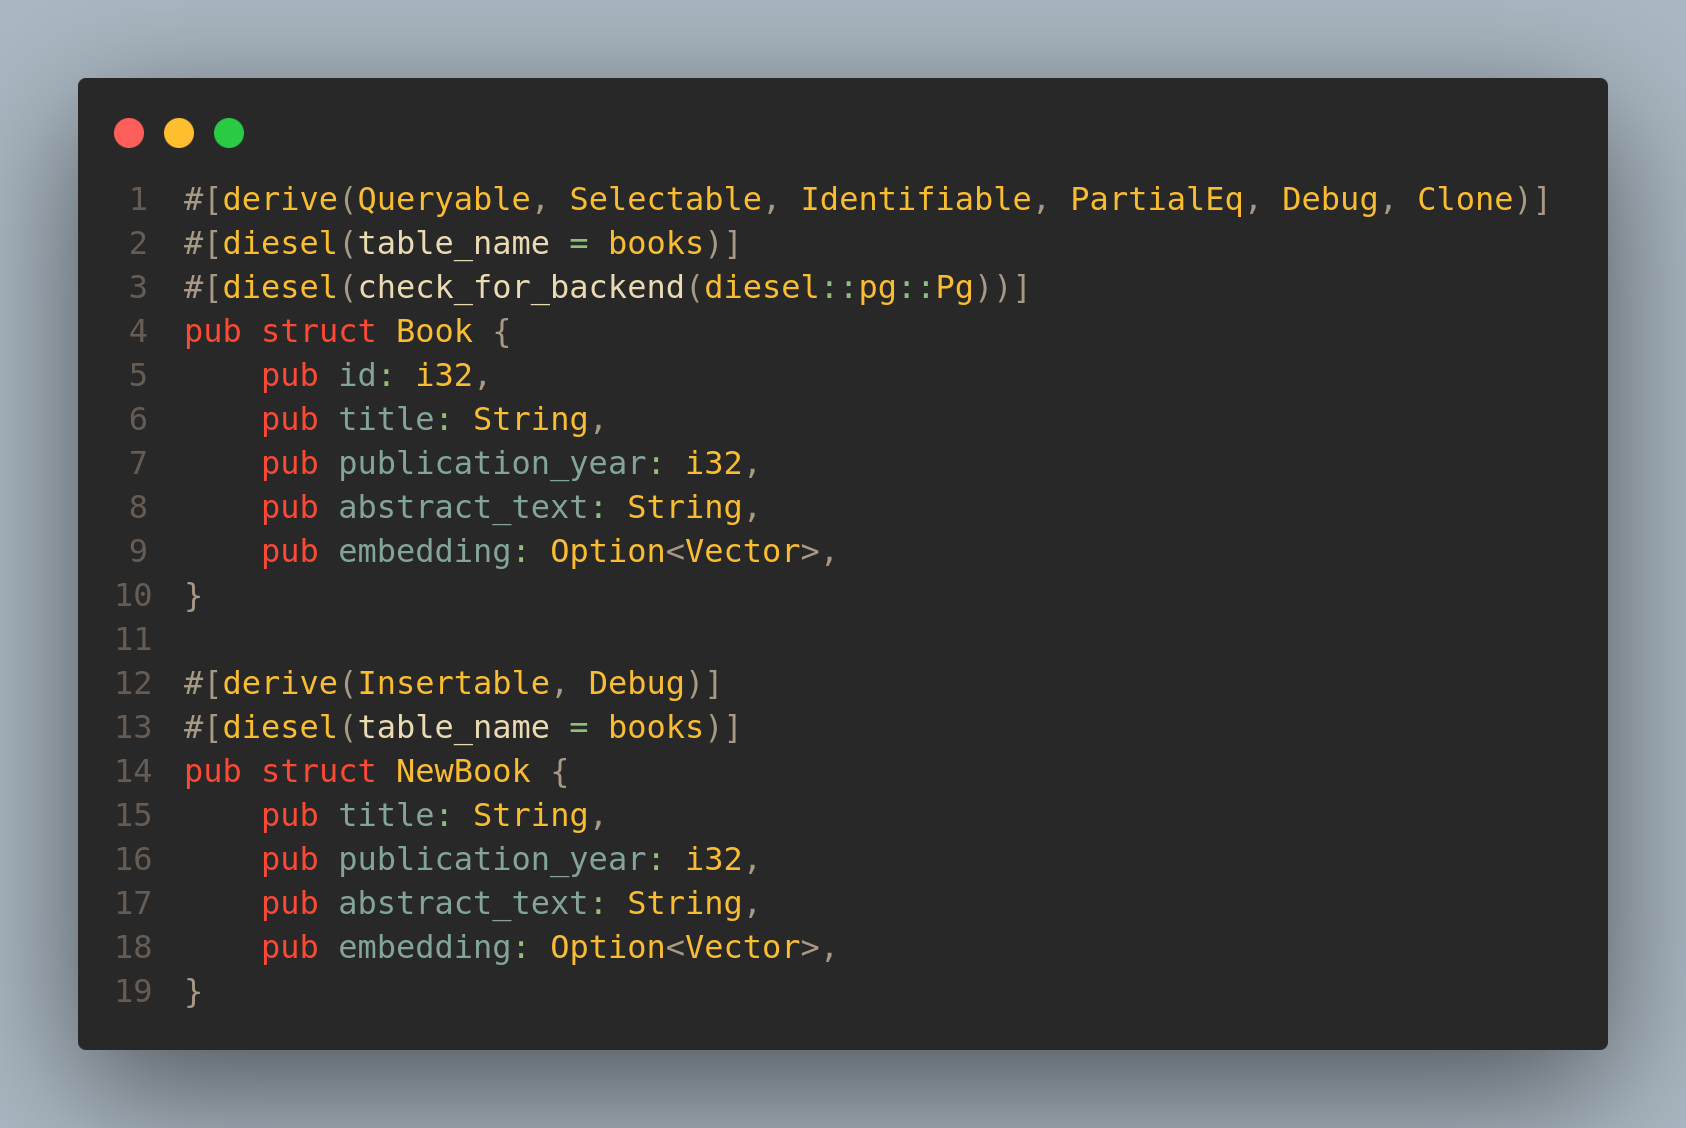
\includegraphics[width=0.9\textwidth]{code.png}
\end{center}
\end{frame}

\begin{frame}{Arquitetura Final do Backend}
\begin{itemize}
\item \textbf{Linguagem:} Rust (performance + segurança de memória)
\item \textbf{Framework Web:} Actix-web (async, alta performance)
\item \textbf{ORM:} Diesel (type-safe, compile-time checks)
\item \textbf{Banco de Dados:} PostgreSQL + pgvector
\item \textbf{Funcionalidades implementadas:}
    \begin{itemize}
    \item CRUD para autores e livros
    \item Sistema de relacionamentos (N:M)
    \item Busca por similaridade com embeddings
    \item API REST completa
    \end{itemize}
\end{itemize}
\end{frame}

\begin{frame}{Busca Vetorial - Implementação}
\begin{itemize}
\item \textbf{Algoritmo:} N-gram hashing (3-gramas)
\item \textbf{Dimensionalidade:} Vetores de 512 dimensões
\item \textbf{Normalização:} \textit{L2 norm} para consistência
\item \textbf{Métrica de similaridade:} Distância cosseno
\item \textbf{Vantagens:}
    \begin{itemize}
    \item Busca semântica (não apenas palavras-chave)
    \item Performance otimizada com pgvector
    \item Implementação leve (sem dependências externas)
    \end{itemize}
\end{itemize}
\end{frame}

\begin{frame}{Cobertura de Testes -  $cargo llvm-cov$}
\begin{center}
\footnotesize
\begin{tabular}{@{}p{3.5cm}rrrrr@{}}
\toprule
\textbf{Módulo} & \textbf{Regions} & \textbf{Cover} & \textbf{Functions} \\
\midrule
database/initialization.rs & 35 & 77.14\% & 5 \\
database/insertion.rs & 275 & 90.18\% & 13 \\
database/query.rs & 328 & 63.41\% & 25 \\
embedding/mod.rs & 103 & \textbf{99.03\%} & 11 \\
lib.rs & 67 & 74.63\% & 10 \\
models/author.rs & 46 & 71.74\% & 9 \\
models/book.rs & 99 & \textbf{90.91\%} & 13 \\
models/book\_author.rs & 29 & 75.86\% & 7 \\
schema.rs & 3 & \textbf{100.00\%} & 3 \\
\midrule
\textbf{TOTAL} & \textbf{985} & \textbf{79.48\%} & \textbf{96} \\
\bottomrule
\end{tabular}
\end{center}

\vspace{0.5cm}
\begin{itemize}
\item \textbf{18 testes} executados com sucesso
\item Módulo de embeddings com cobertura quase perfeita
\item Foco em testes unitários e de integração
\end{itemize}
\end{frame}

\begin{frame}{Endpoints da API REST}
\begin{center}
\begin{tabular}{@{}p{1.5cm}p{4cm}p{4cm}@{}}
\toprule
\textbf{Método} & \textbf{Endpoint} & \textbf{Descrição} \\
\midrule
POST & /insert/author & Cadastrar novo autor \\
POST & /insert/book & Cadastrar novo livro \\
POST & /insert/book-author-link & Vincular livro a autores \\
POST & /search/authors & Buscar autores por nome \\
POST & /search/books & Buscar livros por título \\
POST & /search/author/books & Buscar livros por autor \\
POST & /search/book/embedding & Busca por similaridade \\
\bottomrule
\end{tabular}
\end{center}

\vspace{0.5cm}
\begin{itemize}
\item API completa com CORS habilitado
\item Tratamento robusto de erros
\item Validação de entrada em todos os endpoints
\end{itemize}
\end{frame}

\begin{frame}{Lições Aprendidas}
\begin{itemize}
\item \textbf{Escolha de tecnologias:} Importância de avaliar maturidade e suporte
\item \textbf{Iteração rápida:} Prototipagem permitiu identificar limitações cedo
\item \textbf{Type safety:} Diesel preveniu muitos bugs em tempo de compilação
\item \textbf{Testes:} Cobertura alta nos módulos críticos (embedding, models)
\item \textbf{Documentação:} Tecnologias maduras facilitam desenvolvimento
\end{itemize}
\end{frame}

\begin{frame}{Demonstração}
\begin{center}
{\Large Demonstração do Sistema}
\vspace{1cm}

\textbf{Funcionalidades a demonstrar:}
\begin{itemize}
\item Cadastro de autores e livros
\item Busca tradicional por título/autor
\item Busca por similaridade semântica
\item Visualização de relacionamentos
\end{itemize}
\end{center}
\end{frame}

\begin{frame}
\begin{center}
{\Huge Muito Obrigado!}
\vspace{1cm}

{\Large Perguntas?}
\vspace{1cm}

\textbf{Projeto IcarUSP}\\
Sistema de Catalogação e Busca de Livros
\end{center}
\end{frame}

\end{document}
